

\setlength{\headheight}{27.41803pt}
\chapter{Integration of the PWD12 Sensor into the Weather Station}

\section*{Introduction}

This chapter details the integration process of the Vaisala \gls{pwd12} visibility sensor into the existing weather station system, which already featured a Vaisala WXT536 for meteorological data collection. The integration covered both hardware and software aspects, requiring careful adaptation of the system architecture to support a second sensor with different communication and data characteristics. Emphasis is placed on maintaining modularity, ensuring system reliability, and enabling cloud connectivity through AWS services. The integration not only enhances the scope of environmental data collected, particularly in terms of visibility and present weather conditions, but also strengthens the platform’s value for Unisphere’s flight monitoring and \gls{uas} operations. Each section of this chapter walks through the technical steps, challenges, and solutions involved in enabling seamless communication, data acquisition, offline buffering, and cloud synchronization for the new sensor.

\section{System Architecture and Data Flow}

\subsection{Revised Hardware and Software Stack Overview}

With the integration of the Vaisala \gls{pwd12} sensor, the weather station now incorporates two separate sensing units: the existing WXT536 for core weather measurements and the \gls{pwd12} for visibility and present weather detection. Both sensors are physically connected to the same \gls{revpi} device using dedicated \gls{rs485} serial interfaces. The WXT536 operates at 19200~bps while the \gls{pwd12} uses 9600~bps, which necessitates independent communication ports for reliable operation.

In terms of cabling, the PWD12 is connected to the RevPi through its 8-pin M12 connector. 
Only the essential lines are used: the power supply (24 V DC) and the RS-485 differential 
pair for serial communication. Optional connections such as heater power or analog outputs 
were not required in this deployment and were therefore left unconnected.

Table~\ref{tab:pwd12integrationpins} summarizes the wiring used for the integration, 
while Figure~\ref{fig:pwd12integration} illustrates the simplified pinout layout of the 
8-pin connector as implemented in the weather station.

\begin{table}[H]
\renewcommand{\arraystretch}{1.8}
\centering
\small
\caption{Pin-out connections used for PWD12 integration into the weather station}
\label{tab:pwd12integrationpins}
\begin{tabular}{|c|l|l|l|}
\hline
\textbf{M12 Pin} & \textbf{Wire Color (Cable)} & \textbf{Function} & \textbf{PWD12 Internal Wire} \\
\hline
2 & Brown   & +24 V DC Power & Red \\
\hline
5 & Grey    & RS-485 A (+)   & Brown \\
\hline
7 & Blue    & RS-485 B (-)   & White \\
\hline
8 & Red     & Power GND      & Black \\
\hline
\end{tabular}
\end{table}


\begin{figure}[H]
  \centering
  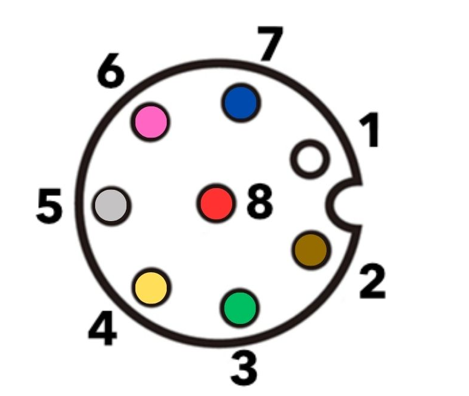
\includegraphics[width=0.45\textwidth]{images/8pins.png}
  \caption{Simplified 8-pin wiring for PWD12 integration into the weather station}
  \label{fig:pwd12integration}
\end{figure}

On the software side, the architecture retains its modular design. Each sensor is handled by its own Python module, responsible for reading, parsing, and structuring messages. These modules run in parallel threads within a single systemd-managed process, ensuring fault isolation and efficient concurrency.

Figure~\ref{fig:hardware_architecture} presents the Updated hardware architecture of the weather station after \gls{pwd12} integration, showing the \gls{revpi} Connect+, dual \gls{rs485} connections (WXT536 and \gls{pwd12}), and supporting power supply.

\begin{figure}[H]
  \centering
  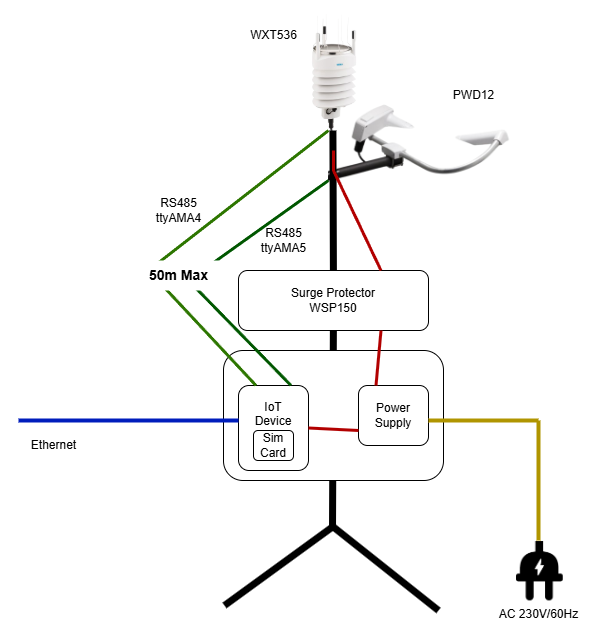
\includegraphics[width=0.75\textwidth]{images/hardware_architecture.png}
  \caption{Revised hardware setup}
  \label{fig:hardware_architecture}
\end{figure}

\subsection{Local Communication and Parsing Workflow}

At the local level, the \gls{revpi} handles real-time communication with both the \gls{pwd12} and WXT536 sensors via two separate \gls{rs485} ports. Each sensor's data stream is processed independently through dedicated reader and parser modules, which are initialized in separate threads within a single Python process managed by systemd. This design ensures that failures in one sensor's parsing logic do not interfere with the operation of the other.

The reader modules continuously monitor their respective serial interfaces, decoding messages based on predefined formats. After basic validation, the data is passed to parser modules that extract relevant fields such as visibility, precipitation, wind speed, or atmospheric pressure. Parsed messages are then structured into unified \texttt{\gls{json}}-like dictionaries and passed downstream for cloud transmission or local buffering.

This modular threading architecture allows for concurrent execution while keeping the codebase maintainable and sensor logic loosely coupled. Figure~\ref{fig:revpi_data_flow} summarizes the local data flow within the \gls{revpi}: independent serial reading threads parse WXT536 and \gls{pwd12} messages into structured \gls{json} dictionaries for either cloud upload or local buffering.

\begin{figure}[H]
  \centering
  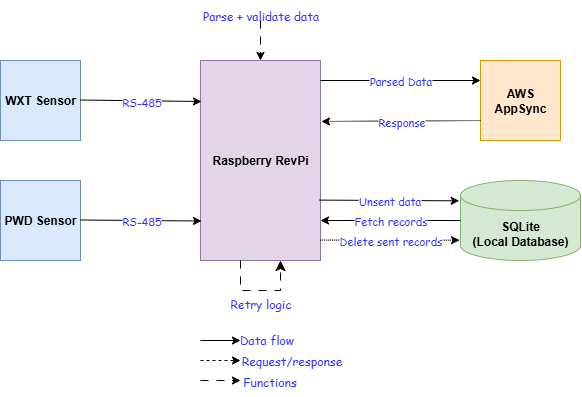
\includegraphics[width=0.7\textwidth]{images/RevPi_data_flow.png}
  \caption{Data flow within the \gls{revpi}: from sensor input to message parsing and output}
  \label{fig:revpi_data_flow}
\end{figure}

\subsection{Cloud Transmission Pipeline and AWS Integration}

Once data is parsed and structured locally, it is transmitted to the cloud via a GraphQL \gls{api} exposed by \gls{aws} appsync. Both the \gls{pwd12} and WXT536 sensors share the same endpoint, with each message tagged by a sensor-specific identifier to allow differentiation on the backend. This unified interface simplifies the cloud integration and reduces the need for multiple endpoints or \gls{api} configurations.

The cloud pipeline relies on \gls{aws} AppSync as the main entry point, forwarding validated messages to a DynamoDB table for temporary storage and to backend services such as Lambda for further processing.

This design enables near real-time access to weather and visibility data while maintaining flexibility for downstream analytics or alerting procedures. The structure also supports asynchronous operations like offline buffering and retry mechanisms, which are detailed later in Section~\ref{sec:offline-buffering}.

\section{Codebase Structure and Development Environment}
\label{sec:codebase-structure}

\subsection{Programming Environment and Tools Used}

The weather station system is developed in \textbf{Python 3.11} and runs on \textbf{Raspberry Pi OS (Bookworm)} installed on the RevPi Connect+. This environment offers a stable and flexible base, with full support for modern Python features and libraries. 

The system relies on a minimal set of external dependencies, declared in a dedicated \texttt{requirements.txt} file. These include modules for serial communication, environment variable loading, GraphQL API interaction, and \gls{json} processing. In addition, runtime and deployment are supported by standard Linux services and external tools for version control and remote management. 

Table~\ref{tab:tools} summarizes the key tools and technologies used, organized by category to reflect their different roles in the system.


\begin{table}[H]
\centering
\small
\caption{Key development tools and technologies}
\label{tab:tools}
\begin{tabular}{|p{5cm}|p{3cm}|p{7.5cm}|}
\hline
\textbf{Category} & \textbf{Tool} & \textbf{Function} \\
\hline
Python Libraries & \texttt{pyserial} & Serial port communication \\
 & \texttt{requests} & HTTP-based GraphQL communication \\
 & \texttt{python-dotenv} & Environment variable loading \\
\hline
System \& Runtime Tools & \texttt{systemd} & Persistent background service management \\
\hline
Deployment \& Remote Management & \texttt{git} & Version control and deployment \\
 & \texttt{Qbee} & Remote access, configuration, and logging \\
\hline
\end{tabular}
\end{table}


\subsection{Folder Layout and Modularization Approach}

The codebase is organized in a modular structure to improve clarity, reusability, and separation of concerns. Each sensor has its own folder containing the core scripts for reading and parsing serial messages. Shared utilities such as offline buffering or main orchestration logic reside in the project root directory.
{\small
\begin{lstlisting}[language=bash,caption={Project folder layout (simplified)},label={lst:folder-structure-ascii}]
    weather_station/
|- docs
|  |- images
|  |- sensor_installation.md
|  |- sensor_specifications.md
|  \- system_architecture.md
|- pwd12/
|  |- error_handler.py
|  |- parser.py
|  \- reader.py
|- wxt536/
|  |- checksum_handler.py
|  |- parser.py
|  \- reader.py
|- buffer_manager.py
|- main.py
|- data_structure.md
|- env_var.env
|- README.md
|- requirements.txt
\- .gitignore
\end{lstlisting}
}



This separation allows sensor-specific logic to be maintained independently, with minimal coupling. Shared logic such as error handling or buffering is centralized to prevent duplication.

\subsection{Environment Variable Management and Secrets Handling}

To avoid hardcoding sensitive information such as \gls{api} keys and serial port paths, the system loads its configuration from a \texttt{.env} file using the \texttt{python-dotenv} package. This approach enables secure and flexible deployments, especially when using version control.
{\small
\begin{lstlisting}[language=bash,caption={Example .env file entries},label={lst:.env}]
APPSYNC_ENDPOINT=https://your-api.appsync-api.amazonaws.com/graphql
APPSYNC_API_KEY=your-secret-key
PWD_ID=IPC2100_PWD12
WXT_ID=IPC2100_WXT536
WXT_PORT=/dev/ttyAMA4
PWD_PORT=/dev/ttyAMA5
\end{lstlisting}
}
These variables are injected at runtime and accessed by the code using standard environment access functions, providing a clean interface between configuration and logic.



\section{Data Acquisition Pipeline}
\label{sec:data_pipeline}

This section describes how sensor data from the WXT536 and \gls{pwd12} devices is acquired, parsed, and structured locally before being forwarded to cloud infrastructure or buffered during offline periods.

\subsection{Serial Port Communication}

The two sensors communicate independently over dedicated \gls{rs485} interfaces, each connected to its own serial port on the \gls{revpi}. The WXT536 operates at 19200 baud with 8 data bits and no parity, while the \gls{pwd12} uses 9600 baud, 7 data bits, even parity, and one stop bit. Serial port parameters are explicitly set using Python's \texttt{pyserial} library at runtime.

The \gls{pwd12} line reader opens the port using environment variables (via \texttt{dotenv}) and waits for newline-terminated messages in blocking mode. The WXT536 reader uses a higher-level class, \texttt{WXT530ASCII}, to issue ASCII-based polling requests and receive either composite or multi-line data messages. Each read loop runs in its own thread, continuously reading and timestamping data from the corresponding port.

\subsection{Message Parsing and Error Handling}

Once data is read from the serial port, each message is validated and parsed.

\begin{itemize}
    \item \textbf{WXT536}: Each multi-line response is parsed individually using a checksum validation function before converting key-value pairs into a structured dictionary. Custom mappings translate sensor codes (e.g., \texttt{Sm=}, \texttt{Ta=}) into descriptive field names like \texttt{wind\_speed\_average} and \texttt{air\_temperature}.
    \item \textbf{\gls{pwd12}}: Each line is first validated for structure and length using a dedicated validator. The parser decodes the byte stream, filters control characters, and maps numeric fields to visibility, precipitation, and present weather codes. External lookup dictionaries are used for translating \gls{nws} character codes and \gls{wmo} numeric codes into human-readable weather descriptions.
\end{itemize}

Errors such as malformed lines, invalid values, or checksum mismatches are logged and do not crash the main pipeline. For the WXT536, retry logic is included to tolerate transient checksum failures (up to 3 attempts).

Figure~\ref{fig:flow-acquisition} illustrates this parsing and validation workflow step by step.

%%%%%%%%%%%%%%%%%%%%%%%%%%%%%%%%%%%%%%%%
% 1. Sensor Data Acquisition
%%%%%%%%%%%%%%%%%%%%%%%%%%%%%%%%%%%%%%%%
\begin{figure}[H]
\centering
\begin{adjustbox}{width=0.8\textwidth}
\begin{tikzpicture}[node distance=2cm]
\node (start) [startstop] {Start};
\node (read) [process, below of=start] {Read serial message from sensor};
\node (check) [decision, below of=read, yshift=-0.5cm] {Valid message?};
\node (discard) [process, right of=check, xshift=6cm] {Discard message};
\node (parse) [process, below of=check, yshift=-2.5cm] {Parse and structure data};
\node (end) [startstop, below of=parse] {Pass to buffering/transmission};

\draw [arrow] (start) -- (read);
\draw [arrow] (read) -- (check);
\draw [arrow] (check.east) -- ++(2,0) -- (discard.west) node[midway, above]{No};
\draw [arrow] (check.south) -- ++(0,-1.3) -- (parse.north) node[midway, right]{Yes};
\draw [arrow] (parse) -- (end);
\end{tikzpicture}
\end{adjustbox}
\caption{Logigram of sensor data acquisition and validation workflow.}
\label{fig:flow-acquisition}
\end{figure}

\subsection{Schema Mapping and Output Structuring}

After parsing, both sensor data dictionaries are augmented with metadata (such as timestamp and sensor ID) and prepared for transmission. The schema used internally aligns with the backend cloud structure and is converted to \gls{json} before being passed to the GraphQL mutation.

For example, a sample output from the PWD12 parser might be structured as shown in Listing~\ref{lst:pwd12-json}.
{\small
\begin{lstlisting}[language=json, caption={Parsed JSON structure from a PWD12 message}, label={lst:pwd12-json}]
{
  "visibility_alarm": "No Alarm",
  "visibility_1min": 1839,
  "visibility_10min": 1505,
  "present_weather_nws": "Light Rain",
  "present_weather_code_inst": "Rain",
  "present_weather_code_15min": "Rain",
  "present_weather_code_1h": "Rain",
  "precip_intensity": 0.33,
  "precip_cumulative": 12.16,
  "snow_sum": 0
}
\end{lstlisting}

}

This structured representation is then either transmitted directly to \gls{aws} AppSync or stored in a local SQLite buffer in case of network unavailability, as described in Section~\ref{sec:offline-buffering}.

The decision process between cloud transmission and local buffering is shown in Figure~\ref{fig:flow-buffering}.

%%%%%%%%%%%%%%%%%%%%%%%%%%%%%%%%%%%%%%%%
% 2. Offline Buffering
%%%%%%%%%%%%%%%%%%%%%%%%%%%%%%%%%%%%%%%%
\begin{figure}[H]
\centering
\begin{tikzpicture}[node distance=2cm]
\node (start) [startstop] {Incoming parsed data};
\node (netcheck) [decision, below of=start, yshift=-0.5cm] {Internet available?};
\node (sqlite) [process, right of=netcheck, xshift=6cm] {Store in local SQLite database};
\node (push) [process, below of=netcheck, yshift=-1.5cm] {Send directly to cloud (AppSync)};
\node (end) [startstop, below of=push] {Done};

\draw [arrow] (start) -- (netcheck);
\draw [arrow] (netcheck.east) -- ++(2,0) -- (sqlite.west) node[midway, above]{No};
\draw [arrow] (netcheck.south) -- ++(0,-1.3) -- (push.north) node[midway, right]{Yes};
\draw [arrow] (push) -- (end);
\end{tikzpicture}
\caption{Logigram of offline buffering with SQLite.}
\label{fig:flow-buffering}
\end{figure}


\section{Offline Buffering and Local Data Resilience}
\label{sec:offline-buffering}

\subsection{Problem Statement and Design Requirements}

In deployments where cellular connectivity may be unstable or unavailable for long durations, the weather station must guarantee data integrity by buffering locally. The buffering mechanism must:

\begin{itemize}
    \item Store all sensor data during internet outages without loss
    \item Automatically retry sending once connectivity is restored
    \item Prevent duplicated uploads
    \item Limit storage usage and clean up old entries if necessary
\end{itemize}

\subsection{Evaluation of Local Storage Options}

Several local buffering mechanisms were considered for storing sensor data during internet outages. Table~\ref{tab:buffering_comparison} summarizes the trade-offs:

\begin{table}[H]
\centering\
\small
\caption{Local storage option comparison for embedded buffering \cite{sqlite-whentouse,sqlite-acid}.}
\label{tab:buffering_comparison}
\begin{tabular}{|p{3.5cm}|p{3cm}|p{4.5cm}|p{4cm}|}
\hline
\textbf{Storage Option} & \textbf{Persistence} & \textbf{Ease of Access} & \textbf{Suitability} \\
\hline
Volatile Memory Buffer & Lost on reboot or crash & Fast, in-memory operations & \textbf{Unsuitable}: not fault-tolerant \\
\hline
Flat File (e.g. \gls{json}) & Persistent & Requires manual parsing, inefficient updates & \textbf{Limited}: simple but hard to manage \\
\hline
SQLite Database & Persistent & Structured, queryable, concurrent-safe & \textbf{Recommended}: lightweight and robust \\
\hline
\end{tabular}
\end{table}


SQLite was chosen for its balance between simplicity and power. Unlike flat files, it offers atomic transactions, concurrent-safe access in a multithreaded system, and efficient indexing and cleanup mechanisms. It also requires no external dependencies and fits well into the embedded constraints of the Raspberry Pi system. SQLite was selected because it is serverless, \acrshort{acid}-compliant, robust against power loss when used with journaling, and well-suited to embedded devices \cite{sqlite-whentouse,sqlite-acid}.



\subsection{Buffer Architecture and File Management}

The buffer is implemented using a single SQLite table named \texttt{sensor\_data}, created during initialization via \texttt{init\_db()}. Each record consists of:

\begin{itemize}
    \item \texttt{id}: Auto-incremented primary key
    \item \texttt{timestamp}: \gls{utc} epoch time when the data was collected
    \item \texttt{sensor\_id}: Unique identifier of the originating sensor
    \item \texttt{payload}: Serialized \gls{json} string of the sensor data
\end{itemize}

Data is inserted using the \texttt{save\_to\_sqlite()} function after every failed upload attempt or when the system detects that there is no internet connection. Records can be printed, counted, or fetched via helper functions for inspection or synchronization purposes.

\subsection{Retry Logic and Recovery Workflow}

A background synchronization thread runs from startup and enforces \acrshort{fifo} ordering (oldest rows first) so that cloud timelines reflect true sampling order. Connectivity is probed via a lightweight \acrshort{dns} socket check to \texttt{8.8.8.8:53}. The workflow is:

\begin{enumerate}
  \item If connectivity is available, fetch a batch of oldest rows (configurable window, default 100).
  \item Attempt upload for each row in order.
  \item On success, delete the row with \texttt{delete\_row\_by\_id()}.
  \item On the first failure, stop the loop and enter backoff before the next attempt.
\end{enumerate}

The retry and recovery procedure is summarized in Figure~\ref{fig:flow-retry}.

%%%%%%%%%%%%%%%%%%%%%%%%%%%%%%%%%%%%%%%%
% 3. Cloud Transmission & Retry (Improved)
%%%%%%%%%%%%%%%%%%%%%%%%%%%%%%%%%%%%%%%%
%%%%%%%%%%%%%%%%%%%%%%%%%%%%%%%%%%%%%%%%
% 3. Cloud Transmission & Retry (Clean arrows)
%%%%%%%%%%%%%%%%%%%%%%%%%%%%%%%%%%%%%%%%
\begin{figure}[H]
\centering
\begin{adjustbox}{width=0.7\textwidth}
    

\begin{tikzpicture}[node distance=14mm]

\node (start) [startstop] {Check buffer for pending data};
\node (exists) [decision, below=of start] {Entries available?};
\node (send) [process, below=18mm of exists] {Attempt upload via AppSync};
\node (retry) [decision, below=of send] {Upload successful?};
\node (remove) [process, below=18mm of retry] {Delete entry from buffer};

\node (idle) [process, right=30mm of exists] {Idle / wait cycle};
\node (waitretry) [process, right=40mm of retry] {Wait / backoff before retry};

% Main vertical flow
\draw [arrow] (start) -- (exists);
\draw [arrow] (exists) -- node[right]{Yes} (send);
\draw [arrow] (send) -- (retry);
\draw [arrow] (retry) -- node[right]{Yes} (remove);

% No-branches to the right
\draw [arrow] (exists.east) -- node[above]{No} (idle.west);
\draw [arrow] (retry.east) -- node[above]{No} (waitretry.west);

% Loops back to start
\draw [arrow] (idle.north) |- (start.east);
\draw [arrow] (waitretry.north) |- (start.east);
\draw [arrow] (remove.west) -| (start.west);

\end{tikzpicture}
\end{adjustbox}
\caption{Logigram of cloud transmission with retry mechanism.}
\label{fig:flow-retry}
\end{figure}



\subsection{Edge Case Handling and Failure Modes}

\paragraph{Duplicate Prevention}

Each record includes a precise timestamp, and the system verifies non-null input values with \texttt{is\_not\_null()} to avoid uploading corrupted or duplicate data. The cloud endpoint (AppSync) uses timestamps and \gls{ttl} fields for consistency and deduplication.

\paragraph{Batching Efficiency}

Although rows are currently uploaded one by one, the buffer structure supports future batching extensions, e.g., sending up to 25 entries at once using a pipeline resolver.

\paragraph{Max Buffer Size and Cleanup}

To prevent unlimited growth, a maximum buffer size is enforced via the \texttt{MAX\_ROWS} constant. Once this threshold is reached, the system deletes the oldest row using the \texttt{cleanup\_table()} function. This keeps disk usage bounded without requiring external intervention.


\section{Cloud Communication and Batch Upload}

\subsection{GraphQL Mutation Design}
The current deployment uses a single-record mutation that ingests one parsed payload at a time. This keeps the resolver simple and aligns with present throughput requirements.
{\small
\begin{lstlisting}[language=bash,caption={GraphQL schema for single-record weather data ingestion},label={lst:graphql-schema}]
input CreateWeatherDataInput {
    created_at: Float!
    weatherstation_id: String!
    weather_data: AWSJSON!
    expiry_date: Int
}

type WeatherData @aws_api_key
              @aws_cognito_user_pools {
    created_at: Float!
    weatherstation_id: String!
    weather_data: AWSJSON!
    expiry_date: Int
}

type Mutation {
    createWeatherData(input: CreateWeatherDataInput!): WeatherData
        @aws_api_key
        @aws_cognito_user_pools
}

type Query {
    getWeatherData(weatherstation_id: String!, created_at: Float!): WeatherData
        @aws_api_key
        @aws_cognito_user_pools
}

type Subscription {
    onCreateWeatherData(weatherstation_id: String): WeatherData
        @aws_subscribe(mutations: ["createWeatherData"])
        @aws_cognito_user_pools
}
\end{lstlisting}
}

\subsection{AppSync Pipeline Resolver for Batching}
Batch submission (e.g., arrays of up to 25 items) can be added later using an AppSync pipeline resolver that validates each item, writes to DynamoDB in a single request, and returns per-item statuses. As the current station traffic does not require batching, this extension is deferred to future work.


\section{Deployment and Monitoring}
\label{sec:deployment-monitoring}

The integrated system was designed for stable operation in a remote or semi-autonomous context, such as a field-deployed weather station. Deployment strategy and observability were key to ensuring reliability and maintainability in real-world conditions.


\subsection{Deployment Strategy for RevPi}

The application is deployed on a Revolution Pi Connect+ running Raspberry Pi OS
(Bookworm). The software stack, implemented in Python~3.11, is maintained entirely
through \textbf{remote deployment}, ensuring that updates and configuration changes
can be applied without physical access to the device. This is critical in operational
environments where the RevPi may be installed in restricted or hard-to-reach
locations.

Remote management is enabled via Qbee.io, which provides secure device access,
configuration distribution, and automated updates. Standard \gls{ssh} access is also
available as a fallback for manual intervention. Together, these mechanisms ensure
that the system can be continuously improved and maintained in the field.

The overall deployment approach follows these principles:
\begin{itemize}
    \item Source code is version-controlled and hosted in a Git repository.
    \item Updates are pulled remotely onto the RevPi via Qbee shell or \gls{ssh}.
    \item The application (\texttt{main.py}) and dependencies are installed in a
          dedicated working directory (e.g., \texttt{/home/revpi/weather\_station}).
    \item Configuration is stored in a local \texttt{.env} file, excluded from version
          control, to allow site-specific customization without code changes.
\end{itemize}

No containerization layer is used in production, as \textbf{systemd services} proved
more reliable for startup control, simpler debugging, and lower resource overhead on
the embedded device. This strategy provides a lightweight, maintainable, and fully
remote deployment workflow, aligning with operational requirements for weather
station installations.

\subsection{Systemd Configuration and Startup Behavior}

The weather station runs as a persistent service managed by \texttt{systemd}, ensuring automatic startup after reboot and consistent recovery after crashes. An example unit file is shown below:

\begin{lstlisting}[language=bash, caption={Systemd unit file for PWD12 weather service}, label={lst:pwd12-service}]
[Unit]
Description=PWD12 Weather Station Service
After=network.target

[Service]
Type=simple
User=unisphere
WorkingDirectory=/home/unisphere/weather_station_iot
ExecStart=/home/unisphere/weather_station_iot/start_pwd12.sh
Restart=always
RestartSec=5

[Install]
WantedBy=multi-user.target
\end{lstlisting}

Key systemd behaviors include:
\begin{itemize}
    \item \texttt{Restart=always} with \texttt{RestartSec=5} prevents downtime after failures.
    \item Logs are captured automatically by \texttt{journald} and persist across reboots.
    \item The service runs as a non-privileged user (\texttt{revpi}).
    \item Secrets are stored in a restricted \texttt{.env} file, excluded from Git.
\end{itemize}

In terms of security:
\begin{itemize}
    \item Only the \texttt{unisphere} user has execution permissions.
    \item Environment variables are stored in \texttt{.env}, which is excluded from version control via \texttt{.gitignore}.
    \item The \texttt{start\_pwd12.sh} script is non\-world\-readable.
\end{itemize}

\paragraph{Operational hardening.}
The service is sandboxed using \texttt{NoNewPrivileges=true} and\\  \texttt{PrivateTmp=true}, reducing attack surface. Scripts such as \texttt{start\_pwd12.sh} are non-world-readable, and environment variables are never written to logs.



\subsection{Remote Access and Diagnostics}

Remote management is handled via Qbee.io, which provides secure access for software updates, service restarts, and log inspection. In practice, developers can:
\begin{itemize}
    \item Pull updates from Git or deploy patches.
    \item Restart or monitor \texttt{systemd} services.
    \item Inspect logs with \texttt{journalctl -u weather\_station.service}.
    \item Access the device over SSH with restricted user privileges.
\end{itemize}

These capabilities are essential for updating firmware, applying patches, or performing diagnostics without physical access to the deployment site.


\subsection{Logging, Metrics, and Alerting}

Local logging is handled using standard output via \texttt{print()} statements and captured by \texttt{journald}. Logs can be queried by timestamp, filtered by service, and persist across reboots.

While no dedicated metrics or alerting system is integrated at this stage, the existing logging includes:
\begin{itemize}
    \item Sensor readouts with timestamps.
    \item Cloud publishing outcomes (success or buffer fallback).
    \item Checksum errors or parsing failures.
    \item Offline buffering and sync attempts.
\end{itemize}

\paragraph{Future improvements.}
While no dedicated metrics or alerting system is yet deployed, options include:
\begin{itemize}
    \item Lightweight metrics collection via Prometheus node exporter.
    \item Qbee log forwarding to a centralized dashboard.
    \item Cloud-based alerting on repeated failures or buffer overflows.
\end{itemize}

These extensions would enhance observability and long-term operational resilience.


\section{Documentation and Maintainability}
\label{sec:documentation-maintainability}

To ensure the long-term sustainability of the integrated weather station system, particular attention was given to documentation, modular code design, and update processes. These elements facilitate onboarding new developers, performing remote maintenance, and enabling future sensor additions.


\subsection{Developer Documentation and Comments}

The source code is fully commented and structured around dedicated modules per sensor (e.g., \texttt{pwd12/} and \texttt{wxt536/}). Inline documentation follows Python conventions with clear docstrings for functions and classes.

In addition, the project contains:
\begin{itemize}
    \item A \texttt{README.md} with setup instructions and dependencies.
    \item An annotated \texttt{requirements.txt} to specify Python packages.
    \item Clear environment variable usage via a version-controlled \texttt{.env.example} template.
    \item Diagrams that explain hardware connections and data flow.
\end{itemize}

This documentation provides the context necessary to understand the architecture, communication protocol, and operational flow without deep code inspection.


\subsection{Update Strategy and Future Expansion}

Updates are applied using a Git-based workflow and deployed remotely via Qbee. The current strategy involves:
\begin{itemize}
    \item Pulling changes on-device using the Git \acrshort{cli}.
    \item Updating the systemd service if file paths or execution logic change.
    \item Validating new features in a test environment before rollout.
\end{itemize}

The modular structure allows new sensors to be added with minimal changes to the main logic. For example, adding a third sensor would involve:
\begin{itemize}
    \item Creating a new folder for its reader/parser.
    \item Launching a dedicated thread in \texttt{main.py}.
    \item Updating the GraphQL payload format accordingly.
\end{itemize}

This makes the system extensible without requiring a full redesign.


\subsection{Testing Guidelines and Deployment Checklist}

While no formal \acrshort{cicd} pipeline is implemented, informal testing procedures were followed throughout development. These include:
\begin{itemize}
    \item Serial port echo tests to validate physical sensor communication.
    \item Mock data replay from logs to verify parsing logic.
    \item Cloud sync simulations using disconnected environments.
    \item Offline buffering threshold stress tests (e.g., >700 entries).
\end{itemize}

The deployment checklist includes:
\begin{enumerate}
    \item Ensure all environment variables are defined.
    \item Pull latest code and verify permissions (\texttt{chmod +x} scripts).
    \item Reload and restart the relevant systemd service.
    \item Monitor logs with \texttt{journalctl} for sensor and sync activity.
    \item Optionally, trigger a manual cloud sync to verify AppSync connectivity.
\end{enumerate}

These practices provide confidence in stability across both development and production environments.

\subsection{Files to touch when adding a new sensor.}
\begin{enumerate}
  \item Create \texttt{<sensor>/reader.py} and \texttt{<sensor>/parser.py}.
  \item Register a new thread in \texttt{main.py} with sensor ID and port.
  \item Extend shared schema mapping (payload builder) if new fields are introduced.
  \item Add environment keys to \texttt{.env.example} and document in \texttt{README.md}.
  \item (Optional) Add unit/mocked tests for parser edge cases.
\end{enumerate}


\section{Results}

To validate the integration of the Vaisala \gls{pwd12} sensor, several outcomes were captured from both the device logs (via Qbee) and the cloud infrastructure (AWS DynamoDB).

\subsection{Local Logs via Qbee}

Figure~\ref{fig:qbee-logs} shows a snapshot of the live logs captured from the
\gls{revpi} device through Qbee’s remote console. These logs provide direct
feedback on the end-to-end data pipeline, confirming that sensor messages are
correctly acquired, parsed, and published to the cloud.

A typical log entry contains:
\begin{itemize}
    \item The \textbf{timestamp} of the acquisition.
    \item The \textbf{station identifier} (here: IPC2100).
    \item The \textbf{systemd service name} running the process
          (e.g., \texttt{start\_pwd12.sh}).
    \item An \textbf{excerpt of the parsed message}, showing visibility, present
          weather, and precipitation values in JSON-like format.
    \item The corresponding \textbf{AppSync response}, confirming successful
          ingestion into the cloud backend.
\end{itemize}

In addition to sensor data logs, the console also shows \textbf{buffering
events}, for example ``No buffered data,'' which indicate that the system
checked the local SQLite database for unsent entries but found none.

This combination of structured sensor outputs, AppSync acknowledgements, and
explicit buffering events demonstrates both the correctness of the parsing logic
and the resilience of the upload pipeline under Qbee monitoring.

\begin{figure}[H]
  \centering
  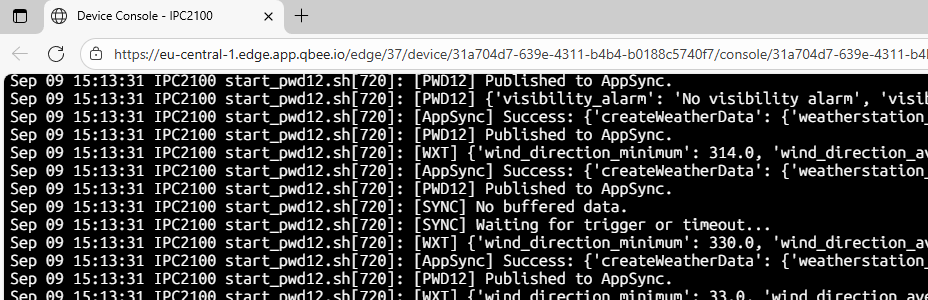
\includegraphics[width=0.9\textwidth]{images/qbee_logs.png}
  \caption{Example of live PWD12 sensor logs captured remotely through Qbee,
           showing parsed data, AppSync responses, and separate buffering events.}
  \label{fig:qbee-logs}
\end{figure}


\subsection{Cloud Data on AWS DynamoDB}

Once parsed and validated, sensor messages are uploaded to the cloud via AppSync and stored in an AWS DynamoDB table. Figure~\ref{fig:dynamodb-table} presents a snapshot of the table view, where each row corresponds to a single data record produced by the weather station. The key attributes visible in this view are the \texttt{created\_at} timestamp (in epoch format) and the \texttt{weatherstation\_id}, which uniquely identify when and where the measurement was taken. The \texttt{weather\_data} field, stored in JSON format, encapsulates the full set of parsed parameters such as visibility averages, present weather codes, precipitation intensity, and snow accumulation. This table therefore represents the chronological archive of all measurements transmitted by the PWD12 sensor, with each record aligned to the structure expected by downstream applications.

\begin{figure}[H]
  \centering
  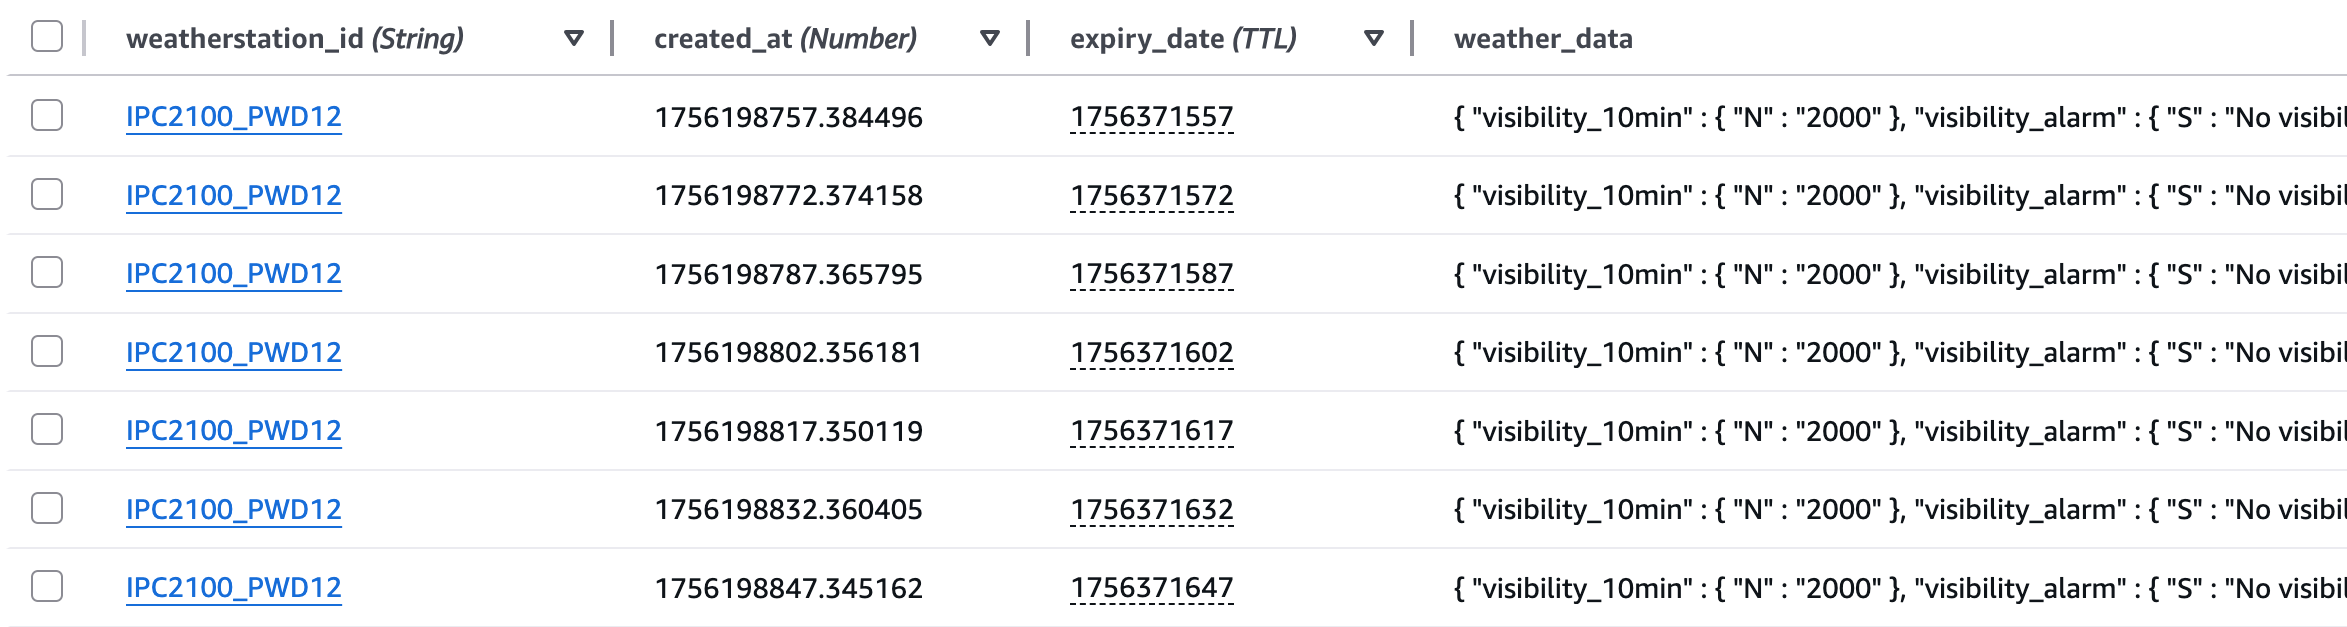
\includegraphics[width=\textwidth]{images/dynamodb_table.png}
  \caption{PWD12 sensor data stored in AWS DynamoDB. Each row corresponds to a structured measurement record with timestamp, station identifier, and JSON payload.}
  \label{fig:dynamodb-table}
\end{figure}

For clarity, Figure~\ref{fig:dynamodb-record} zooms into one specific record. This detailed view highlights how the parsed payload is stored in DynamoDB: the JSON string contains key-value pairs that mirror the structure defined in Section~\ref{sec:data_pipeline}. For example, the fields \texttt{visibility\_1min} and \texttt{visibility\_10min} provide rolling averages of measured visibility, while \texttt{present\_weather\_nws} and \texttt{present\_weather\_code\_inst} capture instantaneous and coded weather conditions. Precipitation values, such as \texttt{precip\_intensity} and \texttt{precip\_cumulative}, are also preserved. In addition, metadata such as the station identifier ensures that data from multiple deployed stations can be distinguished on the backend.

\begin{figure}[H]
  \centering
  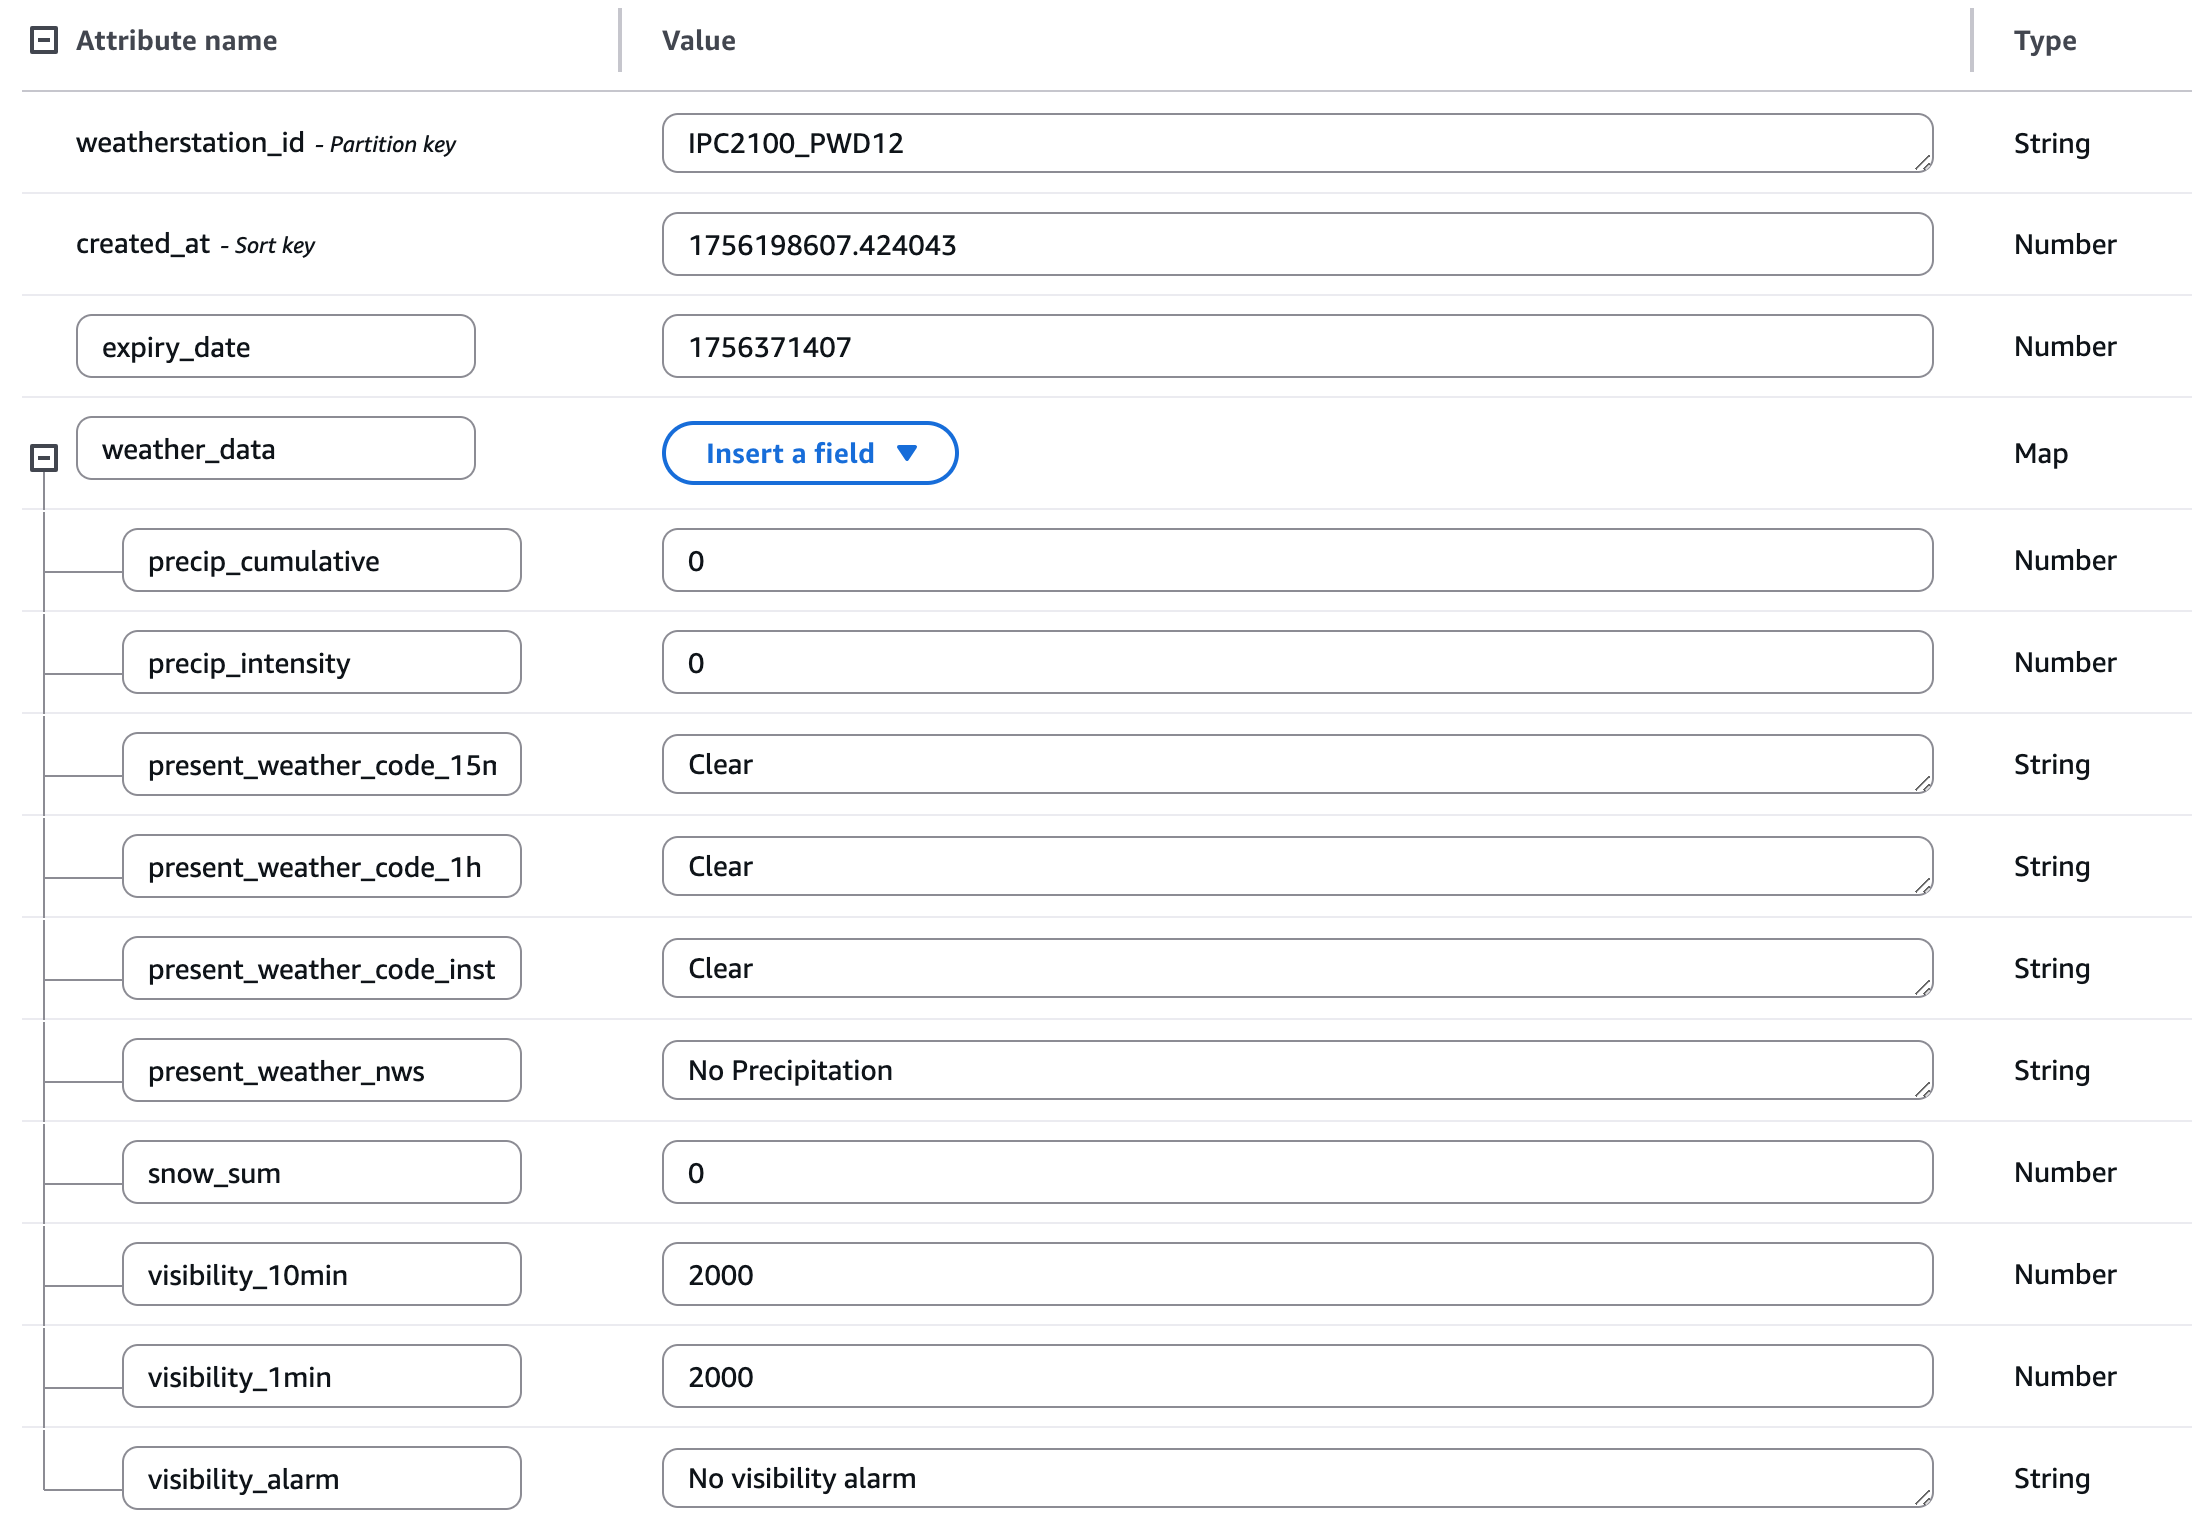
\includegraphics[width=0.85\textwidth]{images/dynamodb_record.png}
  \caption{Detailed view of a single PWD12 sensor record in DynamoDB.}
  \label{fig:dynamodb-record}
\end{figure}

Together, these two figures demonstrate the complete data persistence workflow: sensor messages generated by the PWD12 are parsed locally on the RevPi, buffered when connectivity is unavailable, and then ingested into DynamoDB in a structured format. The result is a reliable, queryable time series of weather data that can be consumed by higher-level services for monitoring, analytics, or flight planning. This confirms both the correctness of the parsing logic and the robustness of the cloud synchronization pipeline.

\subsection{Discussion of Results}

The screenshots illustrate that:
\begin{itemize}
    \item Sensor data is correctly read and parsed on the \gls{revpi}.
    \item Offline buffering and retry logic function as intended when connectivity is intermittent.
    \item Cloud synchronization to AWS AppSync and DynamoDB works reliably, with proper schema mapping and timestamp ordering.
\end{itemize}

These results confirm that the \gls{pwd12} integration provides operational visibility measurements in real-time, both locally and in the cloud, fulfilling the system design objectives.

\subsection{Field Validation and Bug Fixing}

To validate the integration in real-world conditions, the system was temporarily deployed on a rooftop installation in Konstanz. This short-term test allowed direct exposure of the sensors to outdoor weather, providing more realistic operating conditions compared to bench testing. 

During this deployment, several bugs were discovered, primarily related to parsing edge cases and intermittent communication errors. These were fixed iteratively, resulting in a more robust software pipeline capable of handling sensor noise and temporary data gaps. 

No pictures were recorded during this short-term rooftop test, but operational logs and observations confirmed the system’s functionality under real conditions. Representative log excerpts are shown in Figure~\ref{fig:field-validation}, highlighting successful message acquisition, parsing, and cloud transmission.

\begin{figure}[H]
  \centering
  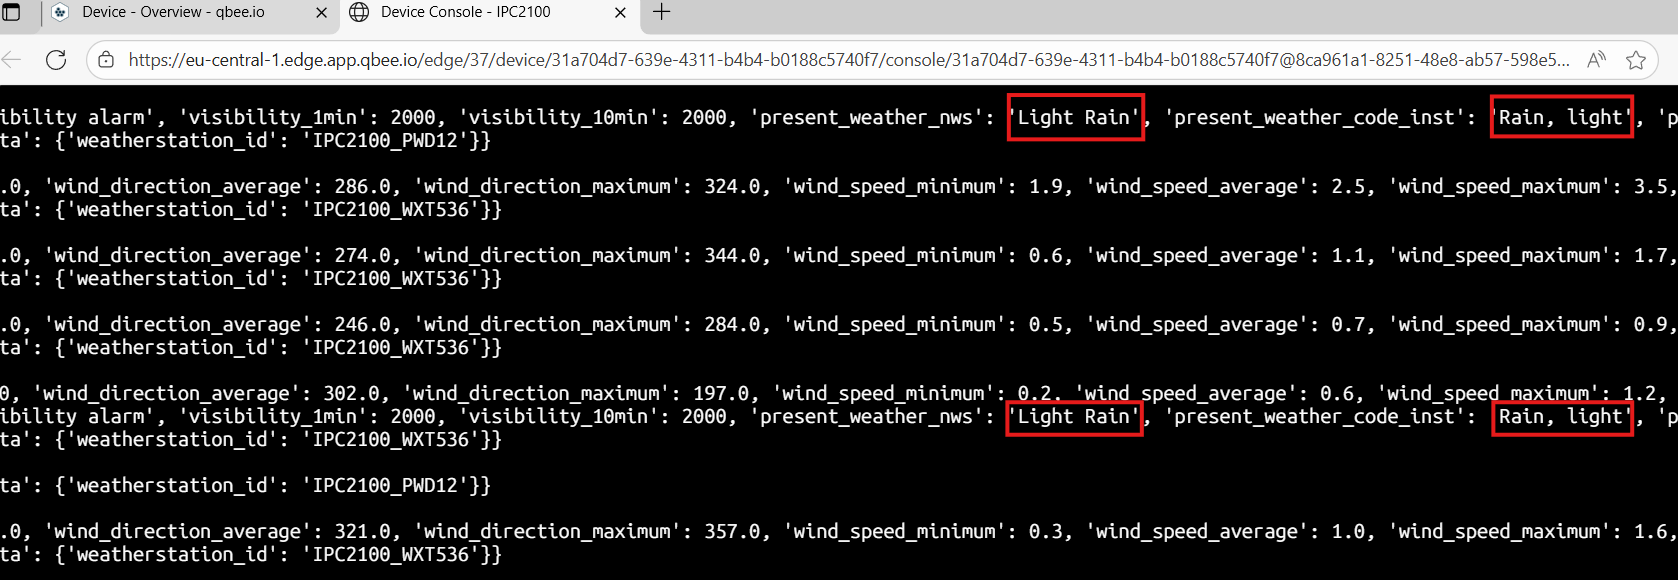
\includegraphics[width=\textwidth]{images/field_test_logs.png}
  \caption{Excerpts from live logs during the rooftop field test.}
  \label{fig:field-validation}
\end{figure}



\section*{Conclusion}

This chapter presented the complete integration of the Vaisala \gls{pwd12} sensor into the existing weather station system. Hardware adaptations enabled stable RS-485 communication, while modular Python components were developed for reading, parsing, and structuring sensor data. Robustness was ensured through local SQLite buffering with retry logic, and cloud synchronization was achieved via AppSync GraphQL mutations. Deployment under systemd provides long-term stability, security, and autonomous operation.



